% ===================================================================
\chapter{Making Sense of the Hardware Numbers}
\label{ch:interpret}

Chapter~\ref{ch:results} reported many hardware numbers: \num{115736} LUTs,
\num{80} block RAMs, \SI{81.88}{\mega\hertz}, \num{61253} cycles and so on.
On their own these are just numbers. A LUT count does not say whether a design
is large or small, and a latency in cycles does not say whether it is fast
enough. Each one needs a yardstick before it means anything.

This chapter supplies the yardsticks. For every metric it answers four
questions, in the same order each time:

\begin{enumerate}
\item \textbf{What does the number physically represent?}
\item \textbf{Why is it measured at all?} Which decision would change if it
were different?
\item \textbf{What should it be compared against?} This is Kiem's design
\cite{kiem2025} where the comparison is like-for-like. Where it is not, the
comparison is against the sensor, the system, the link or the device.
\item \textbf{At what point does it become a problem?}
\end{enumerate}

\noindent
The chapter also corrects three comparisons with the reference design that
earlier drafts of this work got wrong. They are flagged where they occur, and
Table~\ref{tab:kiemvalid} collects them in one place.

\section{Where the numbers come from, and how far to trust them}
\label{sec:numsource}

Not all the numbers in Chapter~\ref{ch:results} are the same kind of number.
Some are exact measurements of the generated circuit; others are estimates the
tool makes before the circuit exists. Table~\ref{tab:numsource} sorts them.

\begin{table}[htbp]
\centering
\caption[Where each hardware number comes from]{Where each hardware number is
read from, and what kind of number it is. \texttt{\emph{top}} is the name of the
design's top-level function. All files are produced by Vitis HLS 2026.1, and
\texttt{collect\_hls\_results.m} reads them all.}
\label{tab:numsource}
\small
\begin{tabular}{@{}p{0.2\textwidth}p{0.33\textwidth}p{0.38\textwidth}@{}}
\toprule
Metric & Read from & What kind of number\\
\midrule
LUT, FF, BRAM, DSP & \texttt{\emph{top}\_csynth.rpt}, top row &
\emph{Estimate} made at C synthesis, before logic optimisation, placement and
routing.\\
$F_{\max}$ & \texttt{\emph{top}\_csynth.xml}, \texttt{EstimatedClockPeriod} &
\emph{Estimate} of the slowest logic path. It includes little or no routing
delay.\\
II, pipeline depth & \texttt{\emph{top}\_csynth.rpt}, loop table &
\emph{Exact} for the generated schedule.\\
Frame latency & \texttt{\emph{top}\_cosim.rpt}, Verilog row &
\emph{Measured}: a cycle-accurate simulation of the generated RTL.\\
Compression ratio & C-simulation and co-simulation logs &
\emph{Measured}: bits out divided by bits in, on real data.\\
\bottomrule
\end{tabular}
\end{table}

\subsection{Synthesis estimates versus implemented figures}

The most important distinction is between an HLS estimate and a
post-implementation figure. After HLS has produced RTL, AMD's Vivado tool
performs three further steps before a design can be loaded onto a chip:
\emph{logic optimisation}, which removes redundant logic and merges duplicated
logic; \emph{placement}, which assigns every element to a physical site on the
chip; and \emph{routing}, which wires the sites together. Only after those steps
are the resource counts and the clock frequency final.

The HLS numbers are made before any of that happens, so they can differ from
the final figures in both directions. LUT and FF counts often come down, because
optimisation removes logic that HLS counted. The achievable clock often comes
down too, because routing adds wire delay that HLS estimated only roughly.

\textbf{Kiem's resource figures are post-implementation; every resource figure
in this thesis is an HLS estimate.} The two are close relatives but not the
same measurement. Comparisons between them are therefore indicative, not exact:
a factor of \num{2.5} in LUTs is a real and meaningful gap, but a
\SI{10}{\percent} difference would not be. The toolchain can close this gap:
\texttt{vitis-run --impl} runs Vivado implementation on the exported design and
produces post-route figures directly comparable with the reference. That run is
listed as future work in Section~\ref{sec:futurework}.

\subsection{What co-simulation measures, and what it does not}

The frame latency from co-simulation is exact for the circuit simulated. It
measures a specific situation, though: the testbench feeds the frame
\emph{back-to-back}, one beat per cycle whenever the design will accept it.
So \num{61253} cycles is the time the compressor would take if an entire frame
were waiting for it at once. The real sensor does not deliver data like that,
which is why Section~\ref{sec:latency} separates this number from the latencies
the system actually experiences.

\section{The yardsticks}
\label{sec:yardsticks}

Six things can give a hardware number meaning:

\begin{enumerate}
\item \textbf{The sensor.} This is how fast data arrives and how much time
passes between ramps and between frames. It sets the throughput requirement.
\item \textbf{The system budget.} This is how long the rest of the processing
chain can afford to wait for compressed data. Kiem derived one explicitly.
\item \textbf{The link.} This is how many bits per second the output
connection can carry. It sets the compression ratio requirement.
\item \textbf{The device.} This is how much of the chip the design uses, and
whether it would fit on a smaller one.
\item \textbf{Kiem's implementation.} This is the only published hardware
DRHE, but it is valid only where the two numbers measure the same thing.
\item \textbf{Internal baselines.} These are the design's own theoretical ideal,
the no-prediction coder, and the entropy bound.
\end{enumerate}

\noindent
Table~\ref{tab:sensoryard} gives the sensor and system figures. They are used
throughout the rest of the chapter.

\begin{table}[htbp]
\centering
\caption[Sensor and system yardsticks]{Sensor and system figures used as
yardsticks. ColoRadar values follow from Table~\ref{tab:capture} and
\cite{kramer2022}. Kiem's values are from his Section~3.3 \cite{kiem2025}.
``Post-FFT'' means the retained half-spectrum as 16-bit complex values, which
is what the compressor receives.}
\label{tab:sensoryard}
\small
\begin{tabular}{@{}lrr@{}}
\toprule
Quantity & ColoRadar cascade & Kiem's sensor\\
\midrule
Range bins per ramp (retained)       & 128 & 512\\
Ramps per frame                      & 192 & 1024\\
Receive channels                     & 16 (4 per compressor) & 4\\
Ramp interval                        & \SI{78.5}{\micro\second} & $\approx$\SI{20.5}{\micro\second}\\
Frame acquisition time               & \SI{15.07}{\milli\second} & $\approx$\SI{21}{\milli\second}\\
Frame period                         & \SI{200}{\milli\second} (\SI{5}{\hertz}) & \SI{50}{\milli\second} (\SI{20}{\hertz})\\
Compression time budget              & --- & \SI{15}{\milli\second}\\
Post-FFT rate, 4 RX, during a frame  & \SI{0.209}{Gbit/s} & \SI{3.20}{Gbit/s}\\
Post-FFT rate, all RX, during a frame& \SI{0.835}{Gbit/s} & \SI{3.20}{Gbit/s}\\
Clock cycles per ramp at \SI{100}{\mega\hertz} & \num{7850} & $\approx$\num{2050}\\
\bottomrule
\end{tabular}
\end{table}

One cross-check is worth recording. Sixteen receive channels, 192 ramps and
256 complex 16-bit samples per ramp is \SI{25.2}{\mega bit} of raw ADC data per
frame, which at \SI{5}{\hertz} is \SI{125.8}{\mega bit\per\second}. The
ColoRadar authors quote \SI{126}{Mbps} for this sensor \cite{kramer2022}. The
sensor model used in this chapter therefore agrees with the published one.

\section{Latency: three different things with the same name}
\label{sec:latency}

``Latency'' means \emph{how long something waits}. The question is always
\emph{what} waits, and for \emph{what}. Three quantities in this project are
called latency, and they answer different questions. Confusing them is the
easiest way to draw a wrong conclusion, including when comparing with Kiem.
Figure~\ref{fig:latscale} puts all of them on one time axis.

\begin{figure}[htbp]
\centering
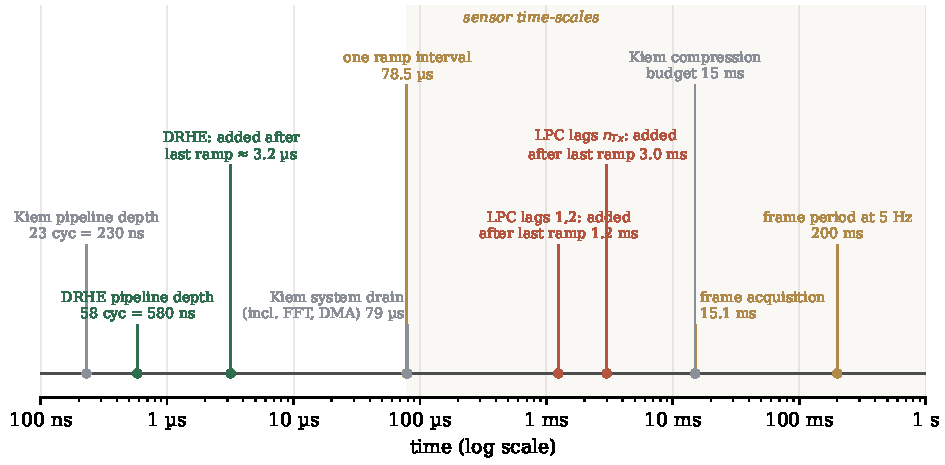
\includegraphics[width=\textwidth]{fig_latency_scale.pdf}
\caption[Latencies on one time axis]{Every latency in this chapter on one
logarithmic time axis. The compressor's own delays (left) are two to five
orders of magnitude shorter than the sensor's time-scales (shaded). The only
compressor delays that approach the sensor's scale are LPC's, because LPC must
see the whole frame before it can emit anything.}
\label{fig:latscale}
\end{figure}

\subsection{Pipeline latency: how long one sample takes to go through}

\paragraph{What it is.} Pipeline latency is the number of clock cycles between
a sample entering the compressor and its compressed bits leaving. For DRHE it
is the pipeline depth, \num{58} cycles, or \SI{580}{\nano\second} at
\SI{100}{\mega\hertz}. Many samples are in flight at once, so this is a delay,
not a rate.

\paragraph{Why measure it.} It fixes two things: how much data is ``inside''
the compressor at any moment, and so how deep any buffering around it must be;
and the smallest possible delay the compressor can add to anything.

\paragraph{Against Kiem: valid.} Kiem reports \SI{230}{\nano\second}, which is
23 cycles. This is his HLS estimate, the same kind of number as ours. He also
measured 31 cycles with an integrated logic analyser, the extra 7 cycles being
the time to fill the first 256-bit output word. Estimate against estimate, this
design is 35 cycles (\SI{350}{\nano\second}) deeper. The cause is known.
Floating-point operators have longer pipelines than fixed-point ones, and the
closed-loop fix of Section~\ref{sec:defect32768} deepened the pipeline from 32
to 58 cycles. That fix is what guarantees the encoder and decoder never
disagree, which Kiem's design does not guarantee.

\paragraph{When does it become a problem?} In this application it does not.
\SI{580}{\nano\second} is \SI{0.7}{\percent} of one ramp interval. It would
matter only in a control loop that must react within about a microsecond, and
no radar perception chain works on that time-scale. The difference from Kiem is
real, but it has no practical consequence here.

\subsection{Frame latency: how long a whole frame takes, if it all arrives at once}

\paragraph{What it is.} Frame latency is the co-simulation figure: \num{61253}
cycles for DRHE, \num{325166} for the corrected LPC. As
Section~\ref{sec:numsource} explained, it is measured with the frame fed
back-to-back. It is really a \emph{throughput} measurement expressed in cycles:
the time to process one frame's worth of work at full speed.

\paragraph{What it is not.} It is not a delay the system ever experiences. The
real sensor delivers a frame over \SI{15.07}{\milli\second}. At
\SI{100}{\mega\hertz} DRHE needs \SI{612.5}{\micro\second} of work to process
it, so the compressor is busy \SI{4.1}{\percent} of the time during a frame. The
rest of the time it waits for the next ramp.

\paragraph{Against Kiem: no equivalent number.} Kiem does not report a
per-frame processing time. His \SI{0.08}{\milli\second} is a different
quantity, discussed next.

\subsection{Added latency: how much later the answer arrives because of compression}
\label{sec:addedlat}

This is the latency that matters to the system, and the right answer to the
question ``what does the latency represent?''

\paragraph{What it is.} Without compression, the downstream processor could
start work on a frame the moment its last ramp had been through the range FFT.
With compression, it must wait until the compressor has emitted the last bit of
that frame. The difference is the \emph{added latency}.

\begin{itemize}
\item \textbf{DRHE} is a streaming design. It processes each ramp as that ramp
arrives, so when the last ramp arrives only that one ramp remains:
\num{319} cycles, or \SI{3.2}{\micro\second} at \SI{100}{\mega\hertz}
(\SI{3.9}{\micro\second} at its estimated $F_{\max}$).
\item \textbf{LPC} cannot emit anything until it has seen the whole frame,
because its coefficients are computed from every ramp. When the last ramp
arrives, it still has all of its solve and emit passes to run. That is
\SI{1.24}{\milli\second} for the baseline and \SI{3.01}{\milli\second} for the
corrected design (\SI{1.45}{} and \SI{3.52}{\milli\second} at $F_{\max}$).
\end{itemize}

\noindent
This is where the two algorithms differ most. DRHE adds microseconds and LPC
adds milliseconds, a factor of about a thousand.

\paragraph{Kiem's \SI{0.08}{\milli\second}: what it measures.} Kiem's system
figure, \SI{79410}{\nano\second}, is measured from the DMA interrupt that
marks the last raw ramp being \emph{read} from memory to the DMA interrupt that
marks the last compressed word being \emph{written} back. That span includes
the range FFT of the last ramp (\num{1787} cycles, \SI{17.9}{\micro\second}),
DMA transfers and interrupt handling as well as the compressor. It is therefore
an \emph{added-latency} measurement for his whole processing chain, not a
compression time and not a per-frame time. This project has no FFT, DMA or
processor in its test system, so it has no measurement of the same span. The
compressor's share of such a span would be the \SI{3.2}{\micro\second} above.
The comparison with \SI{0.08}{\milli\second} should therefore not be made
directly.

\subsection{When does latency become a problem?}
\label{sec:latproblem}

There are three thresholds, from hardest to softest.

\paragraph{1. The throughput threshold: failure.} If the compressor needs
longer to process one ramp than the sensor takes to produce the next one, a
backlog builds up, and no finite buffer can hold it for ever. Data is lost.
This is the only threshold at which the design stops working, so it is the
first to check. For this sensor the limit is \num{7850} cycles per ramp at
\SI{100}{\mega\hertz}. DRHE uses \num{319}, so it would still keep up at a
clock about 25 times slower. LPC's ingest pass runs at one beat per cycle, so
it also keeps up easily. If frames could be buffered whole, the equivalent
limit would be the frame period, \SI{200}{\milli\second}, which both designs
meet by a very wide margin.

\paragraph{2. The budget threshold: the system's schedule.} The downstream
processor must receive each frame in time to finish its own work before the
next frame arrives. Kiem made this explicit for his sensor. It has a
\SI{50}{\milli\second} cycle and \SI{21}{\milli\second} of acquisition, which
leaves \SI{29}{\milli\second}, and he allocated \SI{15}{\milli\second} of that
to compression. For ColoRadar at \SI{5}{\hertz} the gap after acquisition is
about \SI{185}{\milli\second}, and both designs use a tiny fraction of it.

The budget becomes informative when the designs are \emph{scaled to Kiem's
sensor}, whose frame is 21 times larger (512 bins by 1024 ramps against 128 by
192):

\begin{itemize}
\item \textbf{DRHE} still processes one ramp at a time. At 512 bins and
$\mathrm{II} = 2$ a ramp takes about \num{1090} cycles, or
\SI{10.9}{\micro\second}, against a ramp interval of about
\SI{20.5}{\micro\second}. It keeps up, and its added latency stays in
microseconds.
\item \textbf{LPC}'s post-ingest passes scale with the frame. Scaling the
measured cycle counts gives roughly \SI{53}{\milli\second} of added latency
at \SI{100}{\mega\hertz}, which is \emph{3.5 times over} Kiem's
\SI{15}{\milli\second} budget. Its frame buffer would need
\SI{67}{\mega bit}. That exceeds the entire block RAM of the ZU3EG
(\SI{8.0}{\mega bit}) and of the \texttt{xcku5p} (\SI{17.7}{\mega bit}), so
it would have to move to external DRAM.
\end{itemize}

\noindent
So on ColoRadar, LPC's latency is acceptable. On a longer-frame sensor like
Kiem's it is the limiting factor, and it is the strongest argument for DRHE in
this thesis. The scaled figures are extrapolations from measured cycle counts,
not measurements. They are accurate enough to show the budget is exceeded,
because the margin is large.

A related, quieter problem is \emph{double buffering}. If one frame follows
another with no idle gap, LPC is still emitting frame $k$ while frame $k+1$ is
arriving. It then needs a second frame buffer, doubling its largest cost.
DRHE has no frame buffer to double.

\paragraph{3. The application threshold: reaction time.} Finally, any added
delay lengthens the time between something happening in front of the vehicle
and the vehicle knowing about it. A physical scale helps. At
\SI{100}{\kilo\metre\per\hour} a car travels \SI{2.78}{\centi\metre} per
millisecond. LPC's \SI{3.0}{\milli\second} is \SI{8.4}{\centi\metre} of
travel. DRHE's \SI{3.2}{\micro\second} is under a tenth of a millimetre. Both
are small next to the frame period itself: a \SI{5}{\hertz} radar is already
up to \SI{200}{\milli\second}, or \SI{5.6}{\metre}, behind reality. Added
latency becomes an application problem when it is a noticeable fraction of the
frame period. LPC on ColoRadar is \SI{1.5}{\percent}, so it is not a problem.
LPC scaled to Kiem's sensor would exceed his entire \SI{50}{\milli\second}
cycle, so it is.

\section{Throughput and initiation interval}
\label{sec:thrinterp}

\paragraph{What they are.} Throughput is how many bits per second the
compressor can accept. Initiation interval (II) is how many cycles it needs
between accepting one input word and the next. With a 128-bit input word at
clock $f$, the \emph{theoretical} throughput is $128 f / \mathrm{II}$. The
\emph{measured} throughput is the bits in a frame divided by the co-simulated
frame time, and is lower because of pipeline fill and drain.

\paragraph{Why measure it.} Throughput tells us whether the compressor keeps
up with the sensor, which is the throughput threshold of
Section~\ref{sec:latproblem}. II is the main thing that sets throughput, and it
is the thing a designer can change.

\begin{table}[htbp]
\centering
\caption[Throughput: measured, theoretical and required]{Throughput in decimal
Gbit/s. ``Measured'' is from co-simulation, including fill and drain;
``theoretical'' is $128 f / \mathrm{II}$. Kiem's figure is theoretical: his
\SI{11.92}{\gibi bit\per\second} is \SI{12.8}{Gbit/s}.}
\label{tab:thrinterp}
\small
\begin{tabular}{@{}lrrr@{}}
\toprule
& Theoretical & Measured & bits/cycle (meas.)\\
\midrule
DRHE, \SI{100}{\mega\hertz}, $\mathrm{II}=2$       & 6.40 & \textbf{5.136} & 51.4\\
DRHE at $F_{\max}$ (\SI{81.88}{\mega\hertz})       & 5.24 & 4.205 & 51.4\\
LPC lags 1,2, frame average                         & --- & 1.595 & 15.9\\
LPC lags $n_{\mathrm{Tx}}$, frame average           & --- & 0.967 & 9.7\\
Any design at $\mathrm{II}=1$, \SI{100}{\mega\hertz} & 12.80 & --- & 128\\
Kiem \cite{kiem2025}                               & 12.80 & not reported & ---\\
\midrule
\emph{Required:} ColoRadar, 4 RX                   & \multicolumn{3}{l}{0.209}\\
\emph{Required:} ColoRadar, all 16 RX              & \multicolumn{3}{l}{0.835}\\
\emph{Required:} Kiem's sensor                     & \multicolumn{3}{l}{3.20}\\
\bottomrule
\end{tabular}
\end{table}

\paragraph{Against Kiem: a correction.} Kiem's \SI{11.92}{Gbit/s} is
calculated as stream width times clock: $128 \times \SI{100}{\mega\hertz}$,
expressed in binary units. It is the rate his design would reach if it accepted
a word every cycle without pause. It is \emph{not} a measured figure. Earlier
drafts of this work compared it against our \emph{measured}
\SI{5.136}{Gbit/s} and reported a gap of 2.5 times. That mixed a theoretical
number with a measured one. Theoretical against theoretical, the gap is exactly
2, which is II~2 against II~1. The remaining \SI{20}{\percent} is per-ramp
pipeline drain. It appears in our measured number, and it would not appear in
Kiem's theoretical one even if his design had it too.

\paragraph{Against the sensor: the comparison that matters.}
Figure~\ref{fig:headroom} shows capacity against requirement. DRHE accepts
data 24.6 times faster than four ColoRadar channels produce it (20 times at
$F_{\max}$). Throughput beyond the requirement does not improve compression.
It is spare capacity, and it can be spent in three ways:

\begin{itemize}
\item \textbf{Time-multiplexing.} One DRHE instance could serve all 16
receive channels with 6.2 times headroom (5.0 at $F_{\max}$), instead of four
instances. It would need four times the state memory, about 320 BRAM\_18K, but
only one set of logic.
\item \textbf{A slower clock.} Dynamic power scales roughly with clock
frequency. A design with 20 times headroom does not need to run at
\SI{100}{\mega\hertz}.
\item \textbf{Larger sensors.} On Kiem's sensor, which needs
\SI{3.2}{Gbit/s}, DRHE's measured \SI{5.1}{Gbit/s} still has 1.6 times
headroom (1.3 at $F_{\max}$).
\end{itemize}

\begin{figure}[htbp]
\centering
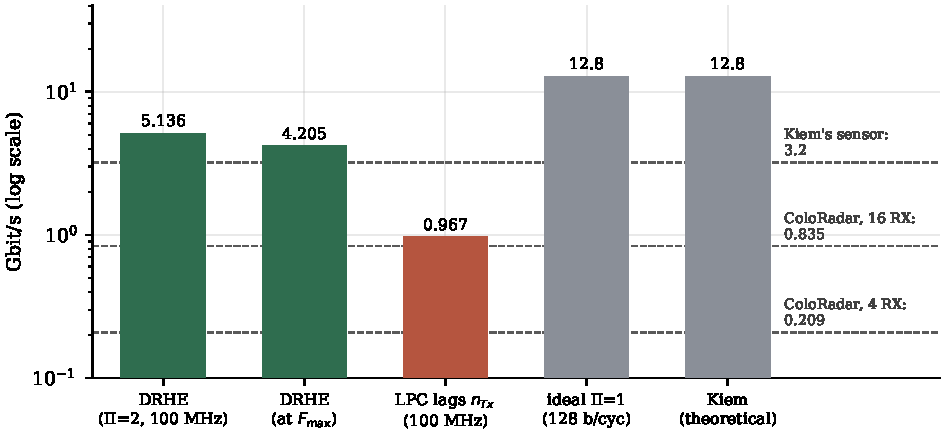
\includegraphics[width=\textwidth]{fig_headroom.pdf}
\caption[Throughput capacity against requirement]{Throughput capacity (bars)
against three requirements (dashed). Capacity above a dashed line is headroom.
DRHE clears every requirement, including Kiem's much faster sensor. The
corrected LPC, measured over a whole frame, clears ColoRadar's full 16-channel
rate only narrowly, which matters only if frames arrive back-to-back.}
\label{fig:headroom}
\end{figure}

\paragraph{Against the architecture's own ideal.} The 128-bit input could in
principle carry 128 bits per cycle. DRHE achieves 51.4, which is
\SI{40}{\percent} of the input width and \SI{80}{\percent} of what II~2 allows.
This is the fairest measure of implementation efficiency, because it needs
nothing external. It also points at the two fixes, the II and the drain,
described in Section~\ref{sec:kiemcompare}.

\paragraph{When does it become a problem?} When headroom falls below 1. For a
single 4-channel ColoRadar stream that would take a design about 25 times
slower than this one. The practical risk is elsewhere. At II~2, the compressor
accepts data at half the rate the FFT core can deliver it within a ramp, so the
FFT must be allowed to pause (AXI back-pressure), or there must be a small
FIFO between them. One ramp for four channels is \SI{16}{\kilo bit}, about one
BRAM\_18K. At II~1 the question would not arise.

\section{Clock frequency}
\label{sec:fmaxinterp}

\paragraph{What it is.} $F_{\max}$ is the fastest clock at which every signal
still settles within one period. It is set by the slowest path in the design,
the critical path. The estimates here are \SI{81.88}{\mega\hertz} for DRHE,
limited by the chain of floating-point transcendental functions, and
\SI{85.43}{\mega\hertz} for LPC.

\paragraph{Why measure it.} Throughput and latency in seconds both depend on
the clock. And the compressor has to run on \emph{some} clock that the rest of
the system provides.

\paragraph{What to compare against.} There are three yardsticks:
\begin{itemize}
\item \textbf{The system clock.} The \SI{100}{\mega\hertz} target is what Kiem
used, and it is a common clock for the programmable logic on these devices.
Kiem met it with fixed-point arithmetic, splitting long operations across
cycles. Neither design here meets it.
\item \textbf{The device.} UltraScale+ logic routinely runs well above
\SI{100}{\mega\hertz} when it is pipelined properly. The
\SI{82}{\mega\hertz} is a limit of the design, not of the chip.
\item \textbf{The requirement.} Section~\ref{sec:thrinterp} showed that
throughput at $F_{\max}$ is still 20 times the requirement.
\end{itemize}

\paragraph{When does it become a problem?} Functionally, only when headroom
at $F_{\max}$ falls below 1, which is far away. In practice, missing
\SI{100}{\mega\hertz} is an \emph{integration} problem rather than a
performance one. If the compressor cannot share the \SI{100}{\mega\hertz}
clock of the FFT and DMA, it needs its own slower clock and a
clock-domain-crossing FIFO on each side. That is standard, but it is extra
design work and extra BRAM. Because the HLS estimate leaves out most routing
delay, the post-route $F_{\max}$ could be lower still, which is one more reason
to run implementation (Section~\ref{sec:numsource}).

\section{Resources: what the design costs}
\label{sec:resinterp}

\paragraph{Why measure resources at all?} Every resource number answers the
same three questions. \emph{Does it fit} on the chip that would actually be
used, next to everything else that chip must do? \emph{What is it costing}
compared with another design that does the same job? And \emph{how does it
scale} when the sensor gets bigger? A design that uses \SI{53}{\percent} of the
chip is a very different proposition from one that uses \SI{5}{\percent}, even
if both work.

Table~\ref{tab:resinterp} compares the resource counts with Kiem's in absolute
terms and as a fraction of both devices.

\begin{table}[htbp]
\centering
\caption[Resources against the reference and against two devices]{Resources of
the two corrected designs against Kiem's compression IP, and as a fraction of
the \texttt{xcku5p} used here and of Kiem's ZU3EG. Kiem's BRAM is converted
from 36\,Kb tiles to BRAM\_18K. Our figures are HLS estimates; Kiem's are
post-implementation.}
\label{tab:resinterp}
\small
\setlength{\tabcolsep}{4pt}
\begin{tabular}{@{}lrrrrrrr@{}}
\toprule
& \multicolumn{2}{c}{Absolute} & & \multicolumn{2}{c}{\% of \texttt{xcku5p}} & \multicolumn{2}{c}{\% of ZU3EG}\\
\cmidrule(lr){2-3}\cmidrule(lr){5-6}\cmidrule(lr){7-8}
& DRHE & LPC & Kiem & DRHE & LPC & DRHE & LPC\\
\midrule
LUT       & \num{115736} & \num{86298} & \num{45892} & 53 & 40 & \textbf{164} & \textbf{122}\\
FF        & \num{57263}  & \num{23154} & \num{9243}  & 13 & 5  & 41 & 16\\
BRAM\_18K & \num{80}     & \num{192}   & \num{20}    & 8  & 20 & 19 & 44\\
DSP       & \num{132}    & \num{156}   & \num{44}    & 7  & 9  & 37 & 43\\
\bottomrule
\end{tabular}
\end{table}

\paragraph{Is comparing absolute counts with Kiem valid?} Mostly yes. Both
devices are AMD UltraScale+ parts on the same process, with the same logic
blocks: a LUT is the same six-input LUT and a DSP is the same DSP48E2 slice.
Absolute counts therefore compare like with like. Percentages do not, because
the \texttt{xcku5p} is three times larger. The one caveat is the HLS-versus-
implementation difference of Section~\ref{sec:numsource}.

\subsection{LUTs}

\paragraph{What they are.} LUTs are the general-purpose logic of the FPGA,
the part that implements every comparison, addition and piece of control logic
that does not go to a dedicated block. The LUT count is the best single
measure of how much \emph{logic} a design is.

\paragraph{What the number says.} DRHE uses 2.5 times Kiem's LUTs, and LPC
1.9 times. The cause is the number format. Kiem wrote his arithmetic in
fixed point. Both designs here use single-precision floating point for the
parts that need it, and DRHE's floating-point square root, arctangent, sine and
cosine are especially expensive. The algorithms are no more complex than
Kiem's; the number format is what costs.

\paragraph{When does it become a problem?} When the design does not fit. At
\SI{164}{\percent} of a ZU3EG's LUTs, DRHE in its current form \emph{could not
be built on Kiem's device at all}, even before the FFT, DMA and processor
interface are added. On their own those used \num{13461} LUTs in Kiem's system
(\num{59353} in total, less \num{45892} for the compressor). A widely used rule
of thumb is also relevant: above about 70--80\,\% utilisation, placement and
routing become congested and timing gets harder to meet. On the
\texttt{xcku5p} DRHE sits at \SI{53}{\percent}, which is comfortable. For the
design to be deployed on a device the size of Kiem's, the float-to-fixed-point
conversion is not optional.

\subsection{Flip-flops}

\paragraph{What they are.} A flip-flop stores one bit from one clock cycle to
the next. Pipelines need them between every pair of stages, so the FF count
mainly reflects \emph{how deeply pipelined} a design is.

\paragraph{What the number says.} DRHE uses 6.2 times Kiem's flip-flops. The
ratio of FFs to LUTs is also informative: 0.49 for DRHE against 0.20 for
Kiem's design. That is what deep floating-point pipelines look like, each
float operator carrying many stages of 32-bit registers.

\paragraph{When does it become a problem?} Rarely. UltraScale+ devices provide
two flip-flops for every LUT, so FFs are seldom the resource that runs out
first. At \SI{13}{\percent} of the \texttt{xcku5p} and \SI{41}{\percent} of a
ZU3EG, they are not the constraint here. They matter indirectly: more
registers switching every cycle means more dynamic power.

\subsection{Block RAM}

\paragraph{What it is.} Block RAM is on-chip memory, counted here in
\SI{18}{\kilo bit} units. It holds anything the design must remember. For
DRHE that is the predictor state, five values per range bin and channel from
previous ramps. For LPC it is mostly the frame buffer.

\paragraph{Against Kiem: a unit correction.} Kiem reports 10 BRAM. His table
counts 36\,Kb tiles (``10 of 216''), not 18\,Kb units. In the unit used here
that is \textbf{20 BRAM\_18K}. Earlier drafts compared our 40 with his 10 and
called it four times as much. The correct ratio for the baseline DRHE is
\textbf{2 times}. That ratio is consistent with storing each state value as a
32-bit float rather than a narrower fixed-point word. With 1024 entries per
array, a 32-bit array fills two BRAM\_18K, where one of 18 bits or fewer fits
in one. The corrected DRHE's 80 is 4 times Kiem's, because it stores twelve
times as many state entries, one set per transmitter.

\paragraph{Against the minimum.} A second yardstick needs no reference design:
how many bits the design \emph{must} store, against how many BRAMs it
occupies. The corrected DRHE must hold $5 \times 4 \times 1536$ 32-bit values,
\SI{0.98}{\mega bit}, or 53.3 BRAM\_18K at perfect packing. It uses 80, about
\SI{67}{\percent} efficiency, because HLS rounds each partitioned array up to
whole BRAMs. LPC's frame buffer is \SI{3.15}{\mega bit}, or 170.7 BRAM\_18K,
and the design uses 192 in total. Both designs use memory sensibly; neither
wastes it.

\paragraph{When does it become a problem?} BRAM is the resource that decides
whether LPC scales. For all 16 ColoRadar channels LPC's frame buffers would
need about 683 BRAM\_18K, \SI{71}{\percent} of the \texttt{xcku5p}. For Kiem's
frame size they would need \SI{67}{\mega bit}, which is more than either device
has (Section~\ref{sec:latproblem}). DRHE's memory scales with the number of
range bins and transmitters, not with the number of ramps, so it never meets
this wall.

\subsection{DSP slices}

\paragraph{What they are.} A DSP slice is a hardened multiplier with an
adder, far cheaper and faster than building a multiplier out of LUTs.
Floating-point multipliers and the arithmetic inside the transcendental
functions consume several each.

\paragraph{What the number says.} DRHE uses 3 times Kiem's DSPs, and LPC 3.5
times. The cause is again floating point: a single-precision multiply needs
several DSP slices where a narrow fixed-point multiply fits in one.

\paragraph{When does it become a problem?} At \SI{7}{\percent} of the
\texttt{xcku5p} and \SI{37}{\percent} of a ZU3EG, not here. DSPs become the
constraint in designs dominated by filtering or FFTs. An FFT sharing the same
device would be the main competitor for them.

\subsection{Scaling to the whole sensor}

The designs compress four receive channels; the sensor has sixteen. There are
two ways to cover all sixteen, and the resource and throughput numbers together
decide between them:

\begin{itemize}
\item \textbf{Four DRHE instances.} This needs \num{462944} LUTs, more than
twice the \texttt{xcku5p}. It does not fit.
\item \textbf{One DRHE instance, time-multiplexed.} Throughput headroom of 6.2
(5.0 at $F_{\max}$) makes this feasible. State memory grows to about 320
BRAM\_18K (\SI{33}{\percent}), while logic stays at one instance.
\end{itemize}

\noindent
This is a good example of why the numbers must be read together. The excess
throughput, which looks like an irrelevant surplus on its own, is exactly what
makes the whole-sensor design fit.

\section{Power: the number not measured}

Power is the metric an automotive integrator would ask about first, and this
thesis does not report it. The reason is that a meaningful power figure needs
the post-implementation design and realistic switching activity. The flow for
that is: Vivado implementation, then \texttt{report\_power} with activity
recorded from co-simulation. An HLS-stage power figure would be too rough to
be worth quoting.

Two things can nonetheless be said. First, power will track the resource
numbers: the floating-point datapath dominates logic, registers and DSPs, so a
fixed-point redesign would reduce power along with area. Second, the
throughput headroom is also a power budget. The same work done at a lower
clock costs proportionally less dynamic power. The right yardstick, when it is
measured, is \emph{energy per compressed bit} against the energy saved by
sending fewer bits over the link.

\section{Compression ratio: what counts as good}
\label{sec:crinterp}

\paragraph{What it is.} Compression ratio (CR) is bits in divided by bits out,
measured on real data. It is the reason the compressor exists.

\paragraph{Against the link.} The link sets the requirement. Kiem's sensor
produces \SI{2.4}{Gbit/s} of raw ADC data. To fit a Gigabit Ethernet link
(1000BASE-T1) it needs a CR of 2.4, or 2.7 once protocol headers are included.
The corrected DRHE's 3.75 would clear that. For ColoRadar the picture is
different, and it should be stated plainly: its post-FFT rate for all 16
channels is \SI{0.835}{Gbit/s} while a frame is being acquired. That already
fits under \SI{1}{Gbit/s}, if only just, before compression. After compression
it is \SI{0.223}{Gbit/s}. On this sensor, compression buys \emph{margin} and
room for more channels, not the ability to use Gigabit Ethernet at all.

\paragraph{Against Kiem: not valid.} Kiem's hardware CR was 3.17, on his own
data. The number looks comparable, but it is not. Section~\ref{sec:decomposition}
showed that 1.63 times of this thesis's ratio comes from unused headroom in the
16-bit container. That is a property of how ColoRadar's data is scaled, not of
the algorithm. A CR measured on a different sensor with different scaling
measures a different thing, so a higher or lower number on another dataset says
nothing about which implementation is better.

\paragraph{The valid yardsticks.} These are the internal ones:
\begin{itemize}
\item \textbf{No prediction.} The same entropy coder applied to the raw values
gives 3.489. This is the test of whether prediction helps at all. The original
designs failed it; the corrected designs beat it by \SI{7.5}{\percent} (DRHE)
and \SI{6.0}{\percent} (LPC).
\item \textbf{The entropy bound.} The order-0 entropy is the least any coder
of this type could spend per value. The fixed Huffman code runs
\SI{6.2}{\percent} above it (Section~\ref{sec:decomposition}), so little is lost
to the coder itself.
\item \textbf{Each other.} DRHE and LPC run on the same data through the same
coder, so their ratios are directly comparable: 3.751 against 3.697.
\end{itemize}

\paragraph{When does it become a problem?} When the compressed rate, plus
protocol overhead, no longer fits the link. The caution from
Section~\ref{sec:decomposition} matters here. A sensor whose ADC output filled
the 16-bit container would lose the 1.63 times headroom factor. A rough
estimate, multiplying the sparsity factor (2.14) by the corrected prediction
gain (1.08), puts its ratio near 2.3, which is \emph{below} the 2.4 Kiem's link
requires. That is an estimate from factors measured on ColoRadar, not a
measurement on such a sensor. It shows that a CR of 3.75 on this dataset is not
a guaranteed pass on every sensor.

\section{Which comparisons with Kiem are valid}

Table~\ref{tab:kiemvalid} collects the conclusions of this chapter about the
reference design.

\begin{table}[htbp]
\centering
\caption[Validity of each comparison with the reference]{Which comparisons with
Kiem's design \cite{kiem2025} are like-for-like, and what to use when they are
not.}
\label{tab:kiemvalid}
\small
\begin{tabular}{@{}>{\raggedright}p{0.13\textwidth}>{\raggedright}p{0.17\textwidth}>{\raggedright}p{0.17\textwidth}>{\raggedright}p{0.09\textwidth}>{\raggedright\arraybackslash}p{0.33\textwidth}@{}}
\toprule
Metric & Kiem & Ours (DRHE) & Valid? & Notes / use instead\\
\midrule
Pipeline latency & 23 cyc (HLS) & 58 cyc (HLS) & Yes &
Both HLS estimates. The gap comes from float pipelines and the closed-loop
fix.\\
Added latency & \SI{79.4}{\micro\second} system & \SI{3.2}{\micro\second} compressor & No &
His includes FFT, DMA and interrupts. Use the system budget
(Section~\ref{sec:latproblem}).\\
Throughput & 12.8 Gbit/s theoretical & 6.4 theor., 5.14 meas. & Partly &
Compare theoretical to theoretical (2 times, from II). Measure both against the
sensor rate.\\
LUT, FF, DSP & post-impl. & HLS est. & Mostly &
Same device family, so absolute counts compare. Percentages do not, because
the devices differ in size. Run \texttt{--impl} to close the gap.\\
BRAM & 10 tiles = 20 BRAM\_18K & 40 (lag 1), 80 (lag $n_{\mathrm{Tx}}$) & Yes, once converted &
2 times, not 4 times, for the baseline.\\
$F_{\max}$ & met \SI{100}{\mega\hertz} (impl.) & \SI{81.88}{\mega\hertz} (est.) & Mostly &
The post-route figure may be lower still.\\
Compression ratio & 3.17 (his data) & 3.75 (ColoRadar) & No &
Different data and scaling. Use the no-prediction baseline and the entropy
bound.\\
\bottomrule
\end{tabular}
\end{table}

\section{Summary: every number, with its yardstick}
\label{sec:interpsummary}

Table~\ref{tab:interpsummary} is the chapter in one table: each headline
number, the yardstick that gives it meaning, and the verdict.

\begin{table}[htbp]
\centering
\caption[Every hardware number with its yardstick]{Each headline number for
the corrected DRHE (LPC where noted), the yardstick it is judged against, and
the verdict.}
\label{tab:interpsummary}
\small
\begin{tabular}{@{}>{\raggedright}p{0.18\textwidth}>{\raggedright}p{0.15\textwidth}>{\raggedright}p{0.27\textwidth}>{\raggedright\arraybackslash}p{0.31\textwidth}@{}}
\toprule
Metric & Value & Yardstick & Verdict\\
\midrule
Throughput & \SI{5.14}{Gbit/s} & \SI{0.209}{Gbit/s} sensor rate & 24.6$\times$ headroom. \textbf{Pass.}\\
Cycles per ramp & 319 & 7850 available & 4\,\% busy. \textbf{Pass.}\\
Pipeline latency & \SI{580}{\nano\second} & \SI{78.5}{\micro\second} ramp & 0.7\,\% of a ramp. \textbf{Irrelevant.}\\
Added latency & \SI{3.2}{\micro\second} & \SI{15}{\milli\second} budget & \textbf{Pass}, including at Kiem's scale.\\
Added latency, LPC & \SI{3.0}{\milli\second} & \SI{15}{\milli\second} budget & Pass here; about \SI{53}{\milli\second} at Kiem's scale. \textbf{Fails there.}\\
$F_{\max}$ & \SI{81.88}{\mega\hertz} & \SI{100}{\mega\hertz} system clock & \textbf{Misses}; needs a clock crossing or a fix.\\
II & 2 & 1 (Kiem, ideal) & Half the ideal. Not needed for this sensor.\\
LUT & \num{115736} & ZU3EG \num{70560}; Kiem \num{45892} & Fits the \texttt{xcku5p}; \textbf{not} the ZU3EG. 2.5$\times$ Kiem.\\
FF & \num{57263} & 2 per LUT on the device & Not a constraint.\\
BRAM\_18K & 80 & Kiem 20; minimum 53 & 4$\times$ Kiem for 12$\times$ the state. Efficient.\\
DSP & 132 & Kiem 44; ZU3EG 360 & 3$\times$ Kiem. Not a constraint.\\
Power & not measured & energy per bit vs.\ link saving & \textbf{Open.}\\
CR & 3.751 & 3.489 no-prediction; 2.7 GbE & Beats the baseline by 7.5\,\%. Data-dependent.\\
\bottomrule
\end{tabular}
\end{table}

\noindent
The overall reading is consistent. \textbf{DRHE meets every
\emph{performance} requirement by a wide margin and misses the \emph{cost} and
\emph{clock} targets set by the reference design.} Both misses have the same
cause, the floating-point datapath, and one known remedy, conversion to fixed
point. LPC is cheaper in logic now, but its latency and memory grow with the
frame. On ColoRadar that is acceptable. On a longer-frame sensor it becomes
the limiting factor.
